\chapter{Технологическая часть}
    В данном разделе рассматривается выбор языка программирования 
    и реализация программного обеспечения.

\section{Выбор языка программирования}
    Операционная система Linux позволяет писать загружаемые модули ядра на Rust и на C.
    Для реализации загружаемого модуля был выбран последний, так как
    большая часть ядра и загружаемых моделей написана на языке C, 
    а также у меня есть опыт разработки модулей на данном языке программирования.

\section{Модификация таблицы системных вызовов}
    Для модификации таблицы системных вызовов 
    требуется изменить данные на странице доступной только для чтения,
    поэтому на время изменения отключается глобальная защита страниц от записи,
    изменением флага WP (Write Protection) в регистре CR0.
    Данные функции представлены в листинге \ref{lst:syscall-hooking:memory}.
    Однако встроенная в Linux функция write\_cr0() не позволяет изменять бит WP, 
    поэтому была реализована своя функция, представленная в листинге \ref{lst:syscall-hooking:cr0_write}.

    \begin{lstlisting}[language=C, label=lst:syscall-hooking:memory, caption=Функции включение и отключение защиты от записи страницы]
#define CR0_WP 0x00010000
static inline void protect_memory(void)
{
    unsigned long cr0 = read_cr0();
    cr0_write(cr0 | CR0_WP);
}

static inline void unprotect_memory(void)
{
    unsigned long cr0 = read_cr0();
    cr0_write(cr0 & ~CR0_WP);
}
    \end{lstlisting}

    \begin{lstlisting}[language=C, label=lst:syscall-hooking:cr0_write, caption=Функция изменения значения регистра cr0]
extern unsigned long __force_order;
inline void cr0_write(unsigned long cr0)
{
    // mov cr0, rax
    asm volatile("mov %0, %%cr0" : "+r"(cr0), "+m"(__force_order));
}
    \end{lstlisting}

    \begin{lstlisting}[language=C, label=lst:syscall-hooking:init, caption=Модификация таблицы системных вызовов]
/* Адрес таблицы системных вызовов */
static unsigned long * __sys_call_table;

static int __init kernel_monitor_init(void)
{
    /* Поиск начального адреса таблицы системных вызовов */
    __sys_call_table = kallsyms_lookup_name("sys_call_table");
    if (!__sys_call_table)
        return -1;

    /* Получение адресов оригинальных системных вызовов */
    orig_open   = (syscall_t)__sys_call_table[__NR_open];
    orig_close  = (syscall_t)__sys_call_table[__NR_close];
    orig_read   = (syscall_t)__sys_call_table[__NR_read];
    orig_write  = (syscall_t)__sys_call_table[__NR_write];
    
    /* Для модификации системной таблицы необходимо снять со страницы защиту от записи */
    unprotect_memory();

    /* Замена системных функций hooks */
    __sys_call_table[__NR_open]     = (unsigned long)hook_open;
    __sys_call_table[__NR_close]    = (unsigned long)hook_close;
    __sys_call_table[__NR_read]     = (unsigned long)hook_read;
    __sys_call_table[__NR_write]    = (unsigned long)hook_write;

    /* Восстановить защиту от записи */
    protect_memory();

    return 0;
}
    \end{lstlisting}

    \begin{lstlisting}[language=C, label=lst:syscall-hooking:exit, caption=Восстановление таблицы системных вызовов]
static void __exit kernel_monitor_exit(void)
{
    /* Восстановление системной таблицы */
    unprotect_memory();
    __sys_call_table[__NR_open]     = (unsigned long)orig_open;
    __sys_call_table[__NR_close]    = (unsigned long)orig_close;
    __sys_call_table[__NR_read]     = (unsigned long)orig_read;
    __sys_call_table[__NR_write]    = (unsigned long)orig_write;
    protect_memory();
}
    \end{lstlisting}

\section{Функции-обёртки перехватываемых системных вызовов}
    На листингах \ref{lst:syscall-hooking:open}-\ref{lst:syscall-hooking:write} 
    представлены реализации функций-обёрток системных вызовов open, close, read, write соответственно.

    \begin{lstlisting}[language=C, label=lst:syscall-hooking:open, caption=Функция-обёртка системного вызова open]
syscall_t orig_open;
asmlinkage int hook_open(const struct pt_regs *regs)
{
    const char __user *filename = (char *)regs->di;
    int flags = (int)regs->si;
    umode_t mode = (umode_t)regs->dx;

    char kernel_filename[NAME_MAX] = {0};

    long error = strncpy_from_user(kernel_filename, filename, NAME_MAX);

    int fd = orig_open(regs);
        
    if (!error && current->real_parent->pid > 3)
        printk(KERN_INFO KERNEL_MONITOR "Process %d; open: %s, flags: %x; mode: %x; fd: %d\n", current->pid, kernel_filename, flags, mode, fd);

    return fd;
}
    \end{lstlisting}

    \begin{lstlisting}[language=C, label=lst:syscall-hooking:close, caption=Функция-обёртка системного вызова close]
syscall_t orig_close;
asmlinkage int hook_close(const struct pt_regs *regs)
{
    unsigned int fd = (unsigned int)regs->di;

    /* Не логировать стандартный ввод/вывод, а так же системные процессы */
    if (fd > 2 && current->real_parent->pid > 3)
    {        
        printk(KERN_INFO KERNEL_MONITOR "Process %d; close fd: %d; filename: %s\n", current->pid, fd, 
            current->files->fdt->fd[fd]->f_path.dentry->d_iname);
    }
    return orig_close(regs);
}
    \end{lstlisting}

    \begin{lstlisting}[language=C, label=lst:syscall-hooking:read, caption=Функция-обёртка системного вызова read]
syscall_t orig_read;
asmlinkage int hook_read(const struct pt_regs *regs)
{
    unsigned int fd = (unsigned int)regs->di;
    char __user *buf = (char*)regs->si;
    size_t count = (size_t)regs->dx;

    /* Не логировать стандартный ввод/вывод, а так же системные процессы */
    if (fd > 2 && current->real_parent->pid > 3)
        printk(KERN_INFO KERNEL_MONITOR "Process %d; read fd: %d; buf: %p; count: %ld; filename: %s\n", current->pid, fd, buf, count,
            current->files->fdt->fd[fd]->f_path.dentry->d_iname);
    return orig_read(regs);
}
    \end{lstlisting}

    \begin{lstlisting}[language=C, label=lst:syscall-hooking:write, caption=Функция-обёртка системного вызова write]
syscall_t orig_write;
asmlinkage int hook_write(const struct pt_regs *regs)
{
    unsigned int fd = (unsigned int)regs->di;
    const char __user *buf = (const char*)regs->si;
    size_t count = (size_t)regs->dx;

    /* Не логировать стандартный ввод/вывод, а так же системные процессы */
    if (fd > 2 && current->real_parent->pid > 3)
        printk(KERN_INFO KERNEL_MONITOR "Process %d; write fd: %d; buf: %p; count: %ld; filename: %s\n", current->pid, fd, buf, count,
            current->files->fdt->fd[fd]->f_path.dentry->d_iname);
    return orig_write(regs);
}
    \end{lstlisting}

\section{Инициализация ftrace}

    \begin{lstlisting}[language=C, label=lst:ftrace-hooking:resolve_hook_address, caption=Поиск адреса функции по символьному имени]
static int fh_resolve_hook_address(struct ftrace_hook *hook)
{
    hook->address = kallsyms_lookup_name(hook->name);

    if (!hook->address)
    {
        printk(KERN_DEBUG "unresolved symbol: %s\n", hook->name);
        return -ENOENT;
    }

    *((unsigned long*) hook->original) = hook->address;
    return 0;
}
    \end{lstlisting}

    \begin{lstlisting}[language=C, label=lst:ftrace-hooking:install_hook, caption=Установка перехвата функции]
int fh_install_hook(struct ftrace_hook *hook)
{
    int err;
    err = fh_resolve_hook_address(hook);
    if(err)
        return err;

    hook->ops.func = fh_ftrace_thunk;
    hook->ops.flags = FTRACE_OPS_FL_SAVE_REGS
            | FTRACE_OPS_FL_RECURSION_SAFE
            | FTRACE_OPS_FL_IPMODIFY;

    err = ftrace_set_filter_ip(&hook->ops, hook->address, 0, 0);
    if(err)
    {
        printk(KERN_DEBUG "ftrace_set_filter_ip() failed: %d\n", err);
        return err;
    }

    err = register_ftrace_function(&hook->ops);
    if(err)
    {
        printk(KERN_DEBUG "register_ftrace_function() failed: %d\n", err);
        return err;
    }

    return 0;
}
    \end{lstlisting}

    \begin{lstlisting}[language=C, label=lst:ftrace-hooking:remove_hook, caption=Отключение перехвата функции]
void fh_remove_hook(struct ftrace_hook *hook)
{
    int err;
    err = unregister_ftrace_function(&hook->ops);
    if(err)
    {
        printk(KERN_DEBUG "unregister_ftrace_function() failed: %d\n", err);
    }

    err = ftrace_set_filter_ip(&hook->ops, hook->address, 1, 0);
    if(err)
    {
        printk(KERN_DEBUG "ftrace_set_filter_ip() failed: %d\n", err);
    }
}
    \end{lstlisting}

\section{Функции-обёртки перехватываемых ftrace функций}
    На листингах \ref{lst:ftrace-hooking:random_read}-\ref{lst:ftrace-hooking:bdev_write_page} 
    представлены реализации функций-обёрток функций random\_read, do\_filp\_open, bdev\_read\_page, bdev\_write\_page соответственно.

    \begin{lstlisting}[language=C, label=lst:ftrace-hooking:random_read, caption=Функция-обёртка функции random\_read]
static asmlinkage ssize_t ( *orig_random_read)(struct file *file, char __user *buf, size_t nbytes, loff_t *ppos);
static asmlinkage ssize_t hook_random_read(struct file *file, char __user *buf, size_t nbytes, loff_t *ppos)
{
    /* Вызов оригинального random_read() */
    int bytes_read;
    bytes_read = orig_random_read(file, buf, nbytes, ppos);
    printk(KERN_INFO KERNEL_MONITOR "Process %d read %d bytes from /dev/random\n", current->pid, bytes_read);
    return bytes_read;
}
    \end{lstlisting}

    \begin{lstlisting}[language=C, label=lst:ftrace-hooking:do_filp_open, caption=Функция-обёртка функции do\_filp\_open]
static asmlinkage struct file* ( *orig_do_filp_open)(int dfd, struct filename *pathname, const struct open_flags *op);
static asmlinkage struct file* hook_do_filp_open(int dfd, struct filename *pathname, const struct open_flags *op)
{
    if (current->real_parent->pid > 3)
        printk(KERN_INFO KERNEL_MONITOR "Process %d; open %s;\n", current->pid, pathname->name);
    
    struct file* file;
    file = orig_do_filp_open(dfd, pathname, op);

    return file;
}
    \end{lstlisting}


    \begin{lstlisting}[language=C, label=lst:ftrace-hooking:bdev_read_page, caption=Функция-обёртка функции bdev\_read\_page]
static asmlinkage int ( *orig_bdev_read_page)(struct block_device *bdev, sector_t sector, struct page *page);
static asmlinkage int hook_bdev_read_page(struct block_device *bdev, sector_t sector, struct page *page)
{
    int err;
    err = orig_bdev_read_page(bdev, sector, page);
    printk(KERN_INFO KERNEL_MONITOR "Process %d bdev_read_page; dev: %d\n", current->pid, bdev->bd_dev);
    return err;
}
    \end{lstlisting}

    \begin{lstlisting}[language=C, label=lst:ftrace-hooking:bdev_write_page, caption=Функция-обёртка функции bdev\_write\_page]
static asmlinkage int ( *orig_bdev_write_page)(struct block_device *bdev, sector_t sector, struct page *page, struct writeback_control *wbc);
static asmlinkage int hook_bdev_write_page(struct block_device *bdev, sector_t sector, struct page *page, struct writeback_control *wbc)
{
    int err;
    err = orig_bdev_write_page(bdev, sector, page, wbc);
    printk(KERN_INFO KERNEL_MONITOR "Process %d bdev_write_page; dev: %d\n", current->pid, bdev->bd_dev);
    return err;
}
    \end{lstlisting}

\section{Примеры работы}

    TODO обновить скрин.
    
    TODO добавить
    прога включилась/выключилась
    прога открыла 1 файл считала 10 байт.
    прога открыла 1 файл, открыла 2ой, закрыла 1ый, закрыла 2ой. 
    1.out
    2.out
    3.out



    На рисунке \ref{3out} представлен пример собранных логов в /var/log/syslog.
    \begin{figure}[h!]
        \centering
        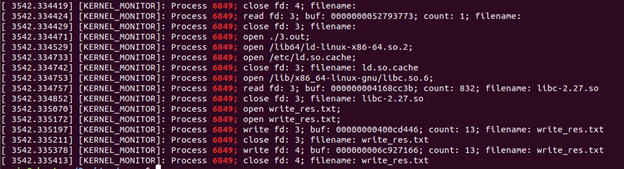
\includegraphics[width = 0.7 \textwidth]{lab_03_3out.png}
        \caption{Пример работы загружаемого модуля ядра.}
        \label{3out}
    \end{figure}

\section{Вывод}
    В данном разделе был обоснован выбор языка программирования, 
    рассмотрены листинги реализованных функций. 
    Приведены результаты работы ПО.

\pagebreak